\section{Công cụ yêu cầu cho bài thí nghiệm}

\subsection{Phần mềm và phần cứng}

\begin{itemize}
    \item Bộ kit Raspberry Pi 3
    \item Màn hình, chuột, bàn phím (tùy chọn)
\end{itemize}

Ta có thể không cần dùng màn hình, chuột, bàn phím 
bằng cách tiền cấu hình tên người dùng, tên miền máy chủ, kết nối mạng... trước khi cài đặt 
và đăng nhập và điều khiển Raspberry Pi từ xa thông qua giao thức SSH hoặc VNC.

\subsection{Giới thiệu bộ kit Raspberry Pi 3}

Các thông số kỹ thuật chính:

{ \centering
\begin{longtable}{rl}
\textbf{Vi xử lý:} & Broadcom BCM2837B0, Cortex-A53 64-bit SoC @ 1.4GHz \\
\textbf{Bộ nhớ:} & 1GB \\
\multirow{4}{*}{\textbf{Kết nối:}} & 2.4 GHz và 5 GHz WLAN \\
 & Bluetooth 4.2 BLE \\
 & Gigabit Ethernet over USB 2.0 \\
 & 4 cổng USB 2.0 \\
\multirow{4}{*}{\textbf{Video và âm thanh:}} & 1 x HDMI kích thước đầy đủ \\
 & Cổng display MIPI DSI \\
 & Cổng camera MIPI CSI \\
 & Ngõ ra stero 4 cực và cổng video composite \\
\multirow{3}{*}{\textbf{Multimedia:}} & H.264, MPEG-4 decode (1080p30) \\
 & H.264 encode (1080p30) \\
 & OpenGL ES 1.1, 2.0 graphics \\
\textbf{Hỗ trợ thẻ SD:} & Thẻ Micro SD cho việc khởi động hệ điều hành và lưu trữ dữ liệu \\
\multirow{2}{*}{\textbf{Nguồn:}} & 5V/2.5A DC qua kết nối micro USB \\
 & 5V DC qua header GPIO \\
\textbf{Nhiệt độ hoạt động:} & 0-50°C
\end{longtable}
}

\begin{figure}[H]
    \centering
    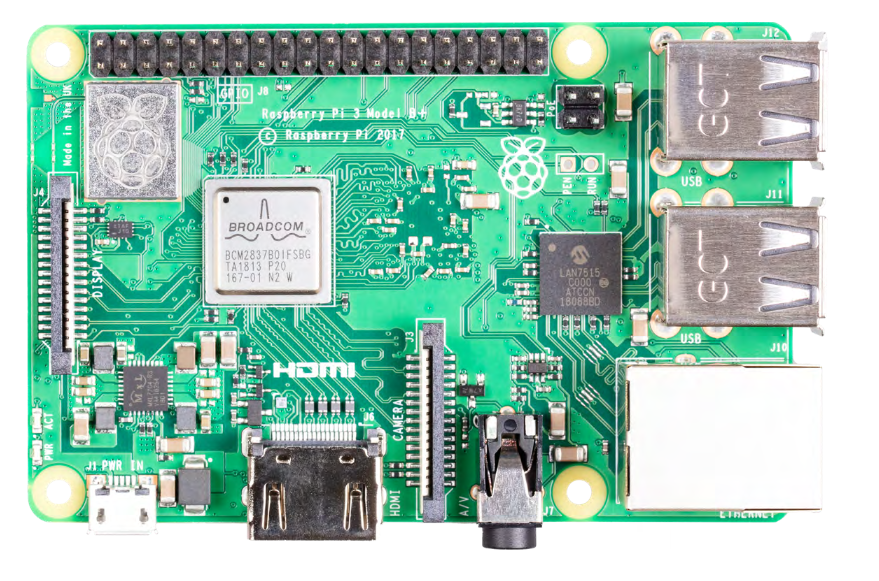
\includegraphics[width=0.75\linewidth]{../images/rpi3.png}
    \caption{Bộ kit Raspberry Pi 3 Model B}
\end{figure}